\section{Обзор существующих моделей}
\label{sec:Chapter2} \index{Chapter2}

\subsection{Модели для распознавания ключевых точек на теле человека}
\label{subsec:pose_estimation_models}

В данном разделе будет рассмотрено 6 различных моделей. В \autoref{sec:Chapter4} будут выбраны 4 наиболее удобные в использовании и в обучении и будет проведен эксперимент по оценке данных моделей.

Так же хочется сказать, что, помимо приведенных, есть множество моделей от одиночных авторов, не объединенных в лаборатории \cite{pet_recognition, pet_classification}. Они в основном брали какую-то из представленных ниже моделей и проводили небольшое улучшение.

А теперь перейдем к моделям.

\subsubsection{BlazePose}
\label{subsubsec:blazepose_desc}

MediaPipe является одним из проектов компании GOOGLE и в своей работе решает задачи компьютерного зрения. В нем уже были представлены модели для распознавания лица (Face Detection) и его поверхности (Face Mesh), ладоней (Hands), объектов (Object Detection и Objectron) и другие \cite{mediapipe}. Для нас же интересна задача поиска ключевых точек, которую и решает модель BlazePose \cite{BlazePose}. На момент исследования модель умеет отслеживать движения человека на видеофрагменте и строить покадровую маску человека.

Для предложенной модели была создана топология, которая представляет собой суперпозицию топологии COCO и двух других топологий, уже использовавшихся в других подпроектах MediaPipe. Об этом более подробно написано в \autoref{subsec:Theory of keypoint detection}.

В BlazePose используется top-down подход оценки позы человека. Сначала запускается Pose Detector (см \autoref{fig:mp_model_structure}), который возвращает координаты интересующей нас области (region-of-interest или ROI). Алгоритм используем расширение модели BlazeFace для определения наличия человека в кадре. Поэтому данная модель чувствительна к видимости головы, лица в частности, на фотографии. Взяв идею витрувианского человека Леонардо Да Винчи, исследователям понадобилось ещё две точки для точной локализации человека на изображении.

\begin{figure}[h]
	\centering
	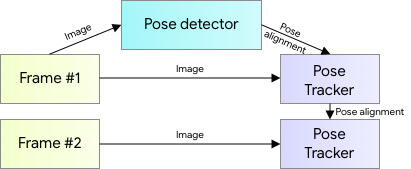
\includegraphics[width=\textwidth * 4 / 5]{./images/MPPose/Model_structure.jpg}
	\caption{Структура модели BlazePose для работы в реальном времени. \cite{BlazePose}}
	\label{fig:mp_model_structure}
\end{figure}

Следующим шагом Pose Tracker производит локализацию каждой точки в заданной ROI. Данное действие производится путем комбинированной обработки тепловой карты и данных о смещении с использованием регрессионной модели (см \autoref{fig:mp_architecture}).

\begin{figure}[h]
	\centering
	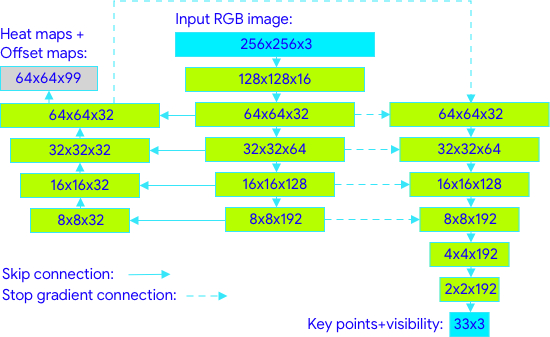
\includegraphics[width=\textwidth * 4 / 5]{./images/MPPose/architecture.jpg}
	\caption{Архитектура модели Pose Tracker. \cite{BlazePose}}
	\label{fig:mp_architecture}
\end{figure}

Как можно заметить из \autoref{fig:mp_model_structure}, при аналитике видеофрагмента Pose Detector используется только на первом кадре, ведь позже данные об интересующей нас области передаются от кадра к кадру. Это упрощает вычисления и позволяет ускорить работу модели в реальном времени.

Развитием данной модели есть ее полное объединение с моделями BlazeFace и BlazeHand в модель Holistic \cite{Holistic}. Она рассматривает намного большее количество точек на лице и ладонях.



\subsubsection{MoveNet.SinglePose}
\label{subsubsec:movenet_desc}

SinglePose создана для работы в веб-интерфейсах или на мобильных устройствах в режиме реального времени. \cite{MoveNet} Модель представлена в двух спецификациях: lightning и thunder. Первая является менее требовательной в плане мощностей и вычислений и способна обрабатывать до 50 кадров в секунду. В то же время, по заверениям создателей, вторая модель имеет большие запросы по ресурсам, но дает лучшую точность распознавания, правда со скоростью до 30 кадров в секунду. 

За расположение ключевых точек выбрана классическая топология COCO. Поэтому модель возвращает координаты 17 точек, которые нормированы на размер изображения (лежат в отрезке [0, 1]).

Представленная модель является восходящей, то есть использует bottom-up подход к решению задачи. Она реализована на архитектуре MobileNetV2 \cite{mobilenetv2} с Feature Pyramid Networks \cite{feature_piramid}, которая используется для извлечения признаков. Обработка результатов магистральной части сети происходит с помощью прогнозирующих головок (см. \autoref{fig:mn_architecture}), которые используют CenterNet \cite{CenterNet} с изменениями, которые повышают быстродействие модели.

\begin{figure}[t]
	\centering
	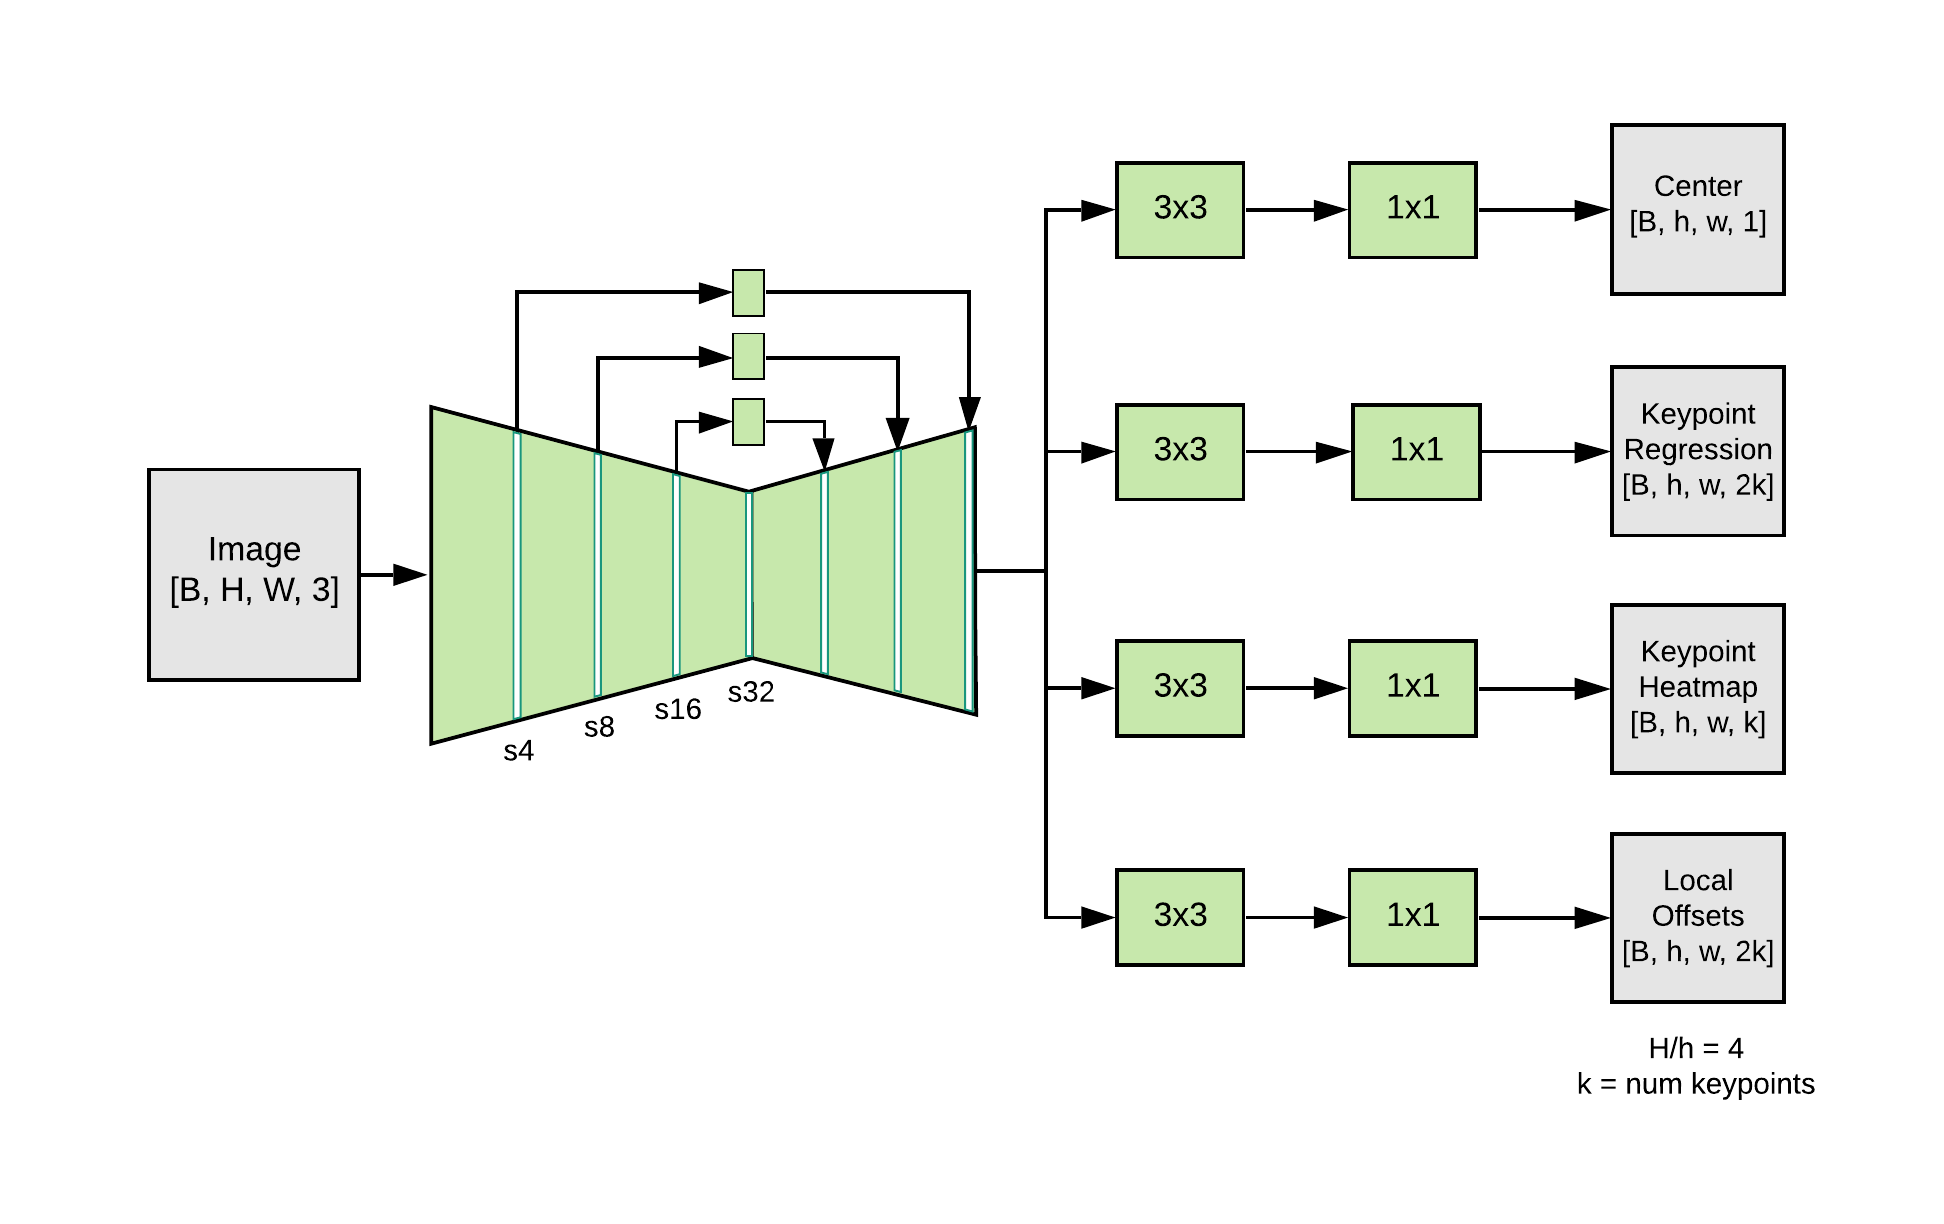
\includegraphics[width=\textwidth * 4 / 5]{./images/MoveNet/architecture}
	\caption{Архитектура модели MoveNet. \cite{MoveNet}}
	\label{fig:mn_architecture}
\end{figure}

Как можно заметить на \autoref{fig:mn_architecture}, 4 прогнозирующие головки отвечают за прогноз карты центральной точки человека, поле регрессионных векторов ключевых точек, карту предсказанных положений ключевых точек и поле смещения ключевых точек. Результаты каждого предсказания вырабатываются параллельно и далее путем последовательной обработки (см. \autoref{fig:mn_structure}) уточняются координаты каждой ключевой точки.

\begin{figure}[h]
	\centering
	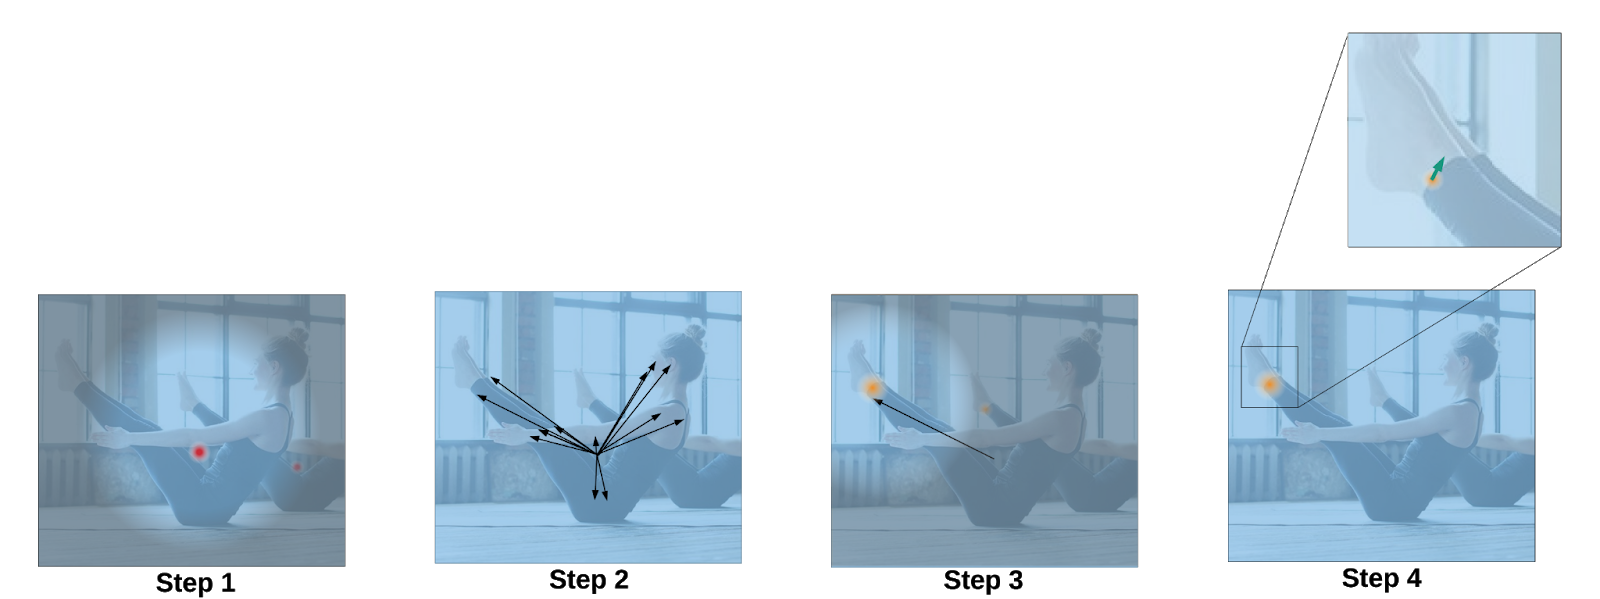
\includegraphics[width=\textwidth * 4 / 5]{./images/MoveNet/structure}
	\caption{Шаги работы prediction head в MoveNet. \cite{MoveNet}}
	\label{fig:mn_structure}
\end{figure}

Такая система позволяет получать точные результаты оценки позы в реальном времени и настроена на обработку в реальном времени изображений, поступающих с камер устройств пользователя.

Следующим этапом развития проекта стала модель MoveNet.MultiPose для распознавания сразу нескольких людей на изображении. Разработчики не стали изменять традициям и представили ее также в двух вариантах: lightning и thunder. А также она использует ту же MobileNetV2 в основе своей работы.



\subsubsection{OpenPose}
\label{subsubsec:openpose_desc}

OpenPose (OP) - это подпроект CMU-Perceptual-Computing-Lab из университета Карнеги-Меллона. В нем представлены различные модели: от локализации точного положения кистей и лица, до определения позы, исследуя 135 точек на теле человека. Также ОР может распознавать нескольких человек одновременно и поддерживает отслеживание скелета человека на видеозаписи в реальном времени через веб-камеру.

В текущей работе рассмотрим модель, работающую по топологии из 25 точек - чем-то похожую на топологию Halpe (см. \autoref{subsec:Theory of keypoint detection}). Особенностью является определение положения стоп за счет детекции 3 дополнительных точек на каждой из них.

OpenPose тоже использует сверточные нейронные сети для решении задачи распознавания ключевых точек с помощью bottom-up подхода. В своей работе исследователи используют понятия карты достоверности обнаружения точки, карты двумерных векторных полей ориентации конечностей (Part Affinity Fields или PAFs) и графы соответствия обнаруженных точек определенным людям на изображении.

Первым шагом происходит обработка изображения и построение карт достоверности и PAFs, про которое поговорим позже. Вторым шагов происходит сопоставление точек и конечностей отдельным людям с использованием графов соответствия. Они помогают решить данную задачу и быстрее решать задачу построения скелетов нескольких человек. В итоге на выходе имеются скелеты нескольких человек. Все шаги представлены на \autoref{fig:op_structure}.

\begin{figure}[t]
	\centering
	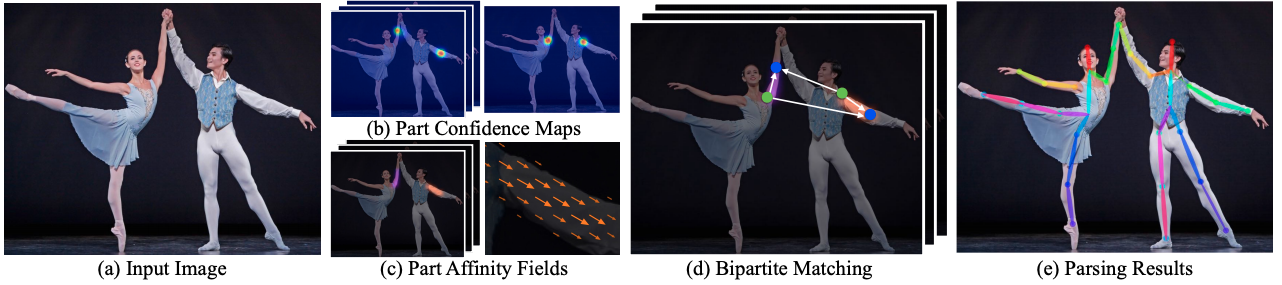
\includegraphics[width=\textwidth]{./images/OpenPose/structure}
	\caption{Последовательность распознавания ключевых точек моделью OpenPose. \cite{OpenPose}}
	\label{fig:op_structure}
\end{figure}

В первоначальной версии модели \cite{OpenPose_first} вычисление карт достоверности и PAFs происходило параллельно, в два этапа. Но в последней работе \cite{OpenPose} предсказания поставили последовательно, так как из PAFs интуитивно можно предсказать и уточнить карты достоверности обнаружения точки (см. \autoref{fig:op_architecture}). Ещё были заменены ядра свертки размером 7х7 на блоки из 3-х последовательных ядер 3х3 (см. \autoref{fig:op_architecture}). Эти преобразование помогло почти в 200 раз увеличить скорость распознавания и в 7 раз улучшить точность.

\begin{figure}[h]
	\centering
	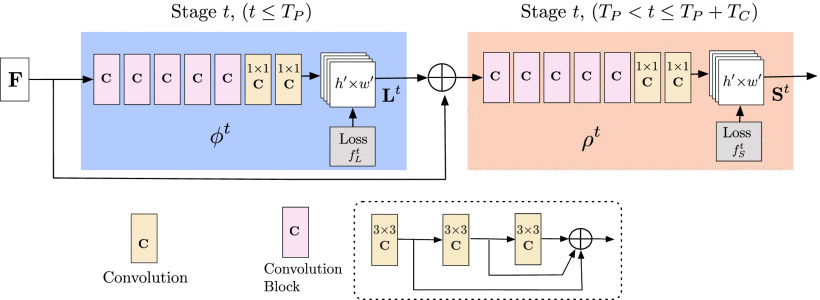
\includegraphics[width=\textwidth * 4 / 5]{./images/OpenPose/architecture.jpg}
	\caption{Архитектура модели OpenPose 2D Pose Estimation. \cite{OpenPose}}
	\label{fig:op_architecture}
\end{figure}



\subsubsection{MMPose}
\label{subsubsec:mmpose_desc}

MMPose - является подпроектом лаборатории Open-MMLab \cite{mmpose2020}. Первым проектом лаборатории было решение задачи детектирования объектов, но позже развивались и другие связанные с компьютерным зрением. Изначально было исследование классификации движений с помощью сетей ST-GCN \cite{STGCN}, но оценку позы решили вынести в отдельную работу. Так появился проект MMPose, включающий в себя распознавание ключевых точек и восстановление скелета человека, модель Animal для тех же задач, но на теле животных. Причем задачи, связанные с человеком, имеют решения с получением предсказаний в 2-х мерном и в 3-х мерном вариантах.

Данная модель постоянно улучшается и подключает новые мировые достижения в свои работы. MMPose использует top-down подход в своей работе и другие наработки лаборатории Open-MMLab. Для работы необходимо сначала использовать detection model, а потом уже передать данные о локализованных людях в pose model.

Детектор натренирован на датасете COCO и выдает предсказания в соответствии с его 17 точечной топологией. Также есть скрипты для обучения на других наборах данных, за что спасибо разработчикам. Правда эти наборы данных надо сначала скачать, но об этом в \autoref{sec:Chapter4}.



\subsubsection{AlphaPose}
\label{subsubsec:alphapose_desc}

AlphaPose является основной наработкой проекта Machine Vision and Intelligence Group из Шанхайского университета транспорта (Shanghai Jiao Tong University или SJTU). Это первая модель, которая получила значение метрики mAP на датасете COCO выше 70 (0.7) и выше 80 на MPII. Поддерживается как на Linux, так и на Windows. Обрабатывает видео и поддерживает слежение за человеком в реальном времени через восстановление его скелета.

Исследователи не против объединяться с другими проектами для улучшения качества модели и проработки новый фичей. Одной из таких коопераций стала топология Halpe (см. \autoref{subsec:Theory of keypoint detection}), на основании которой и производится оценка позы человека. Доступными являются варианты также с 17 точками от COCO и 25 и 135 точек от Halpe.

В работе Alpha использует top-down подход. Первым этапом идет Faster R-CNN для детектирования человека и выдачи прямоугольников. После используется модель RMPE для предсказания различных поз, которые может принимать  человек. Последним этапом идет работа p-Pose NMS для устранению избыточных предсказаний. На выходе получается изображение с восстановленными позами людей. Все шаги представлены на \autoref{fig:ap_structure}. \cite{fang2017rmpe}

\begin{figure}[h]
	\centering
	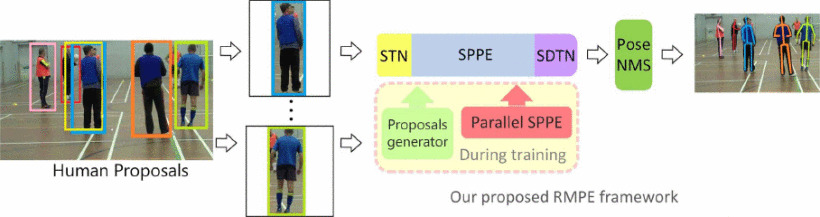
\includegraphics[width=\textwidth]{./images/AlphaPose_structure}
	\caption{Пример работы сети AlphaPose. \cite{fang2017rmpe}}
	\label{fig:ap_structure}
\end{figure}

Рассмотрим поближе модель предсказания. Она использует симметричное преобразование spatial transformer network (STN) и обратное ему spatial de-transformer network (SDTN). Они введены для исправления ошибок локализации, так как SPPE, представленная между ними (см. \autoref{fig:ap_architecture}), является очень чувствительной к неточностям прямоугольника. При обучении параллельно основной модели добавляется ещё одна SPPE (см. \autoref{fig:ap_architecture}) для корректировки преобразования STN. Таким образом получится приблизить данные, получаемые предсказателем, к идеальным и получить наиболее точный результат.

\begin{figure}[t]
	\centering
	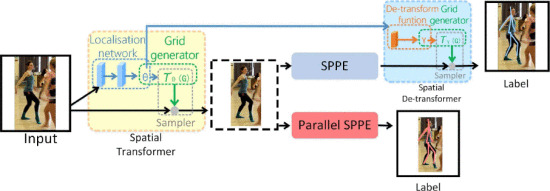
\includegraphics[width=\textwidth]{./images/AlphaPose_architecture}
	\caption{Архитектура сети RMPE. \cite{fang2017rmpe}}
	\label{fig:ap_architecture}
\end{figure}



\subsubsection{DeepPose}
\label{subsubsec:deeppose_desc}

DeepPose является одним из самых первых решений задачи распознавания ключевых точек на теле человека с помощью глубокого обучения. Статья "DeepPose: Human Pose Estimation via Deep Neural Networks"{} \cite{DeepPose} была представлена исследователями из GOOGLE на конференции CVPR в 2014 году.

В своей работе они представили каскад из DNN-регрессоров для локализации суставов тела. На тот момент принятых топологий ещё не было и поза кодировалась координатами суставов, нормализованными на размер изображения.
Первым этапом применялась CNN для локализации точки, а вторым каскадом применялись DNN для уточнения результата (см. \autoref{fig:dp_architecture}). Таким образом получалось довольно точно распознавать ключевые точки на фотографии.

\begin{figure}[h]
	\centering
	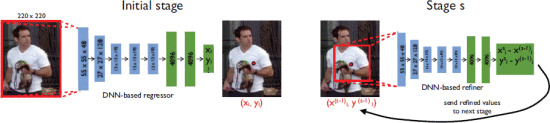
\includegraphics[width=\textwidth]{./images/DeepPose}
	\caption{Архитектура сети DeepPose. \cite{DeepPose}}
	\label{fig:dp_architecture}
\end{figure}
\hfill \break






\subsection{Модели для классификации позы человека}
\label{subsec:pose_classification_models}

Далее будет представлено рассмотрение 4 различных модели, которые можно использовать для классификации движений человека.



\subsubsection{Классификатор от MediaPipe}
\label{subsubsec:mp_classificator_desc}

Проект представил модель для оценки позы человека (см. \autoref{subsubsec:blazepose_desc}) и, добавив к нему k-NN, получили алгоритм классификации позы человека. Таким образом MediaPipe представило программу для счета приседаний или отжиманий с камеры смартфона в реальном времени. \cite{mediapipe_cls}

Для работы использовалась топология BlazePose, а точнее вектор расстояний между некоторыми точками этой топологии (см. \autoref{fig:blazepose_classificator}). Так как в реальных изображениях бывают разные масштабы и размеры, то все позы нормализуются и переориентируются в вертикальное положение.

\begin{figure}[h]
	\centering
	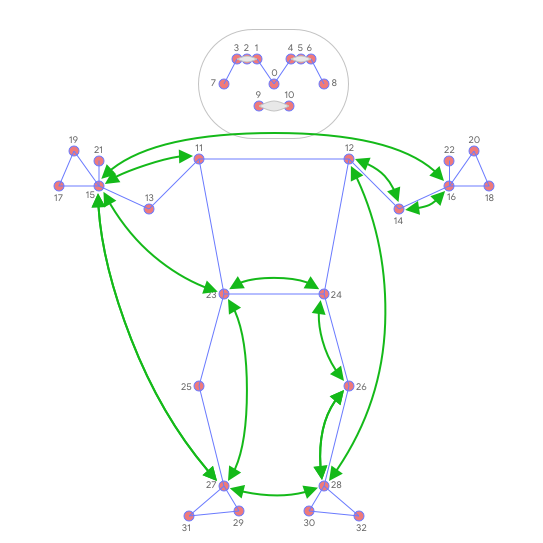
\includegraphics[width=0.6\textwidth]{./images/Classificators/BlazePose}
	\caption{Расстояния между точками топологии BlazePose, которые используются в классификации. \cite{mediapipe_cls}}
	\label{fig:blazepose_classificator}
\end{figure}

Для обеспечения точности классификации разработчики решили запускать k-NN дважды: первый раз для отбора векторов признаков для похожих с целевой поз, а во второй раз для отбора точной позы среди выбранных ранее. Различия в том, что используются различные метрики минимальное покоординатное расстояние и среднее покоординатное расстояния для первого и второго прогона соответственно.



\subsubsection{mmakos}
\label{subsubsec:mmakos_desc}

Модель является бакалаврской работой студента Варшавского университета Михала Макоса \cite{mmakos}. Классификатор работает с видеоданными и разделяет модели на два супер класса: статические и динамические.

Разработчик взял за основу модель распознавания позы человека OpenPose (см. \autoref{subsubsec:openpose_desc}) и преобразовал входные данные из 4-х мерного формата в 2-мерное изображение (см. \autoref{fig:mmakos_image_prep}). По сути три координаты каждой ключевой точки преобразовывались в BGR формат и создавался столбец пикселей для текущего момента времени. При рассмотрении 15 точек и 32 кадров получаются переходные изображения размером (15, 32, 3).

\begin{figure}[h]
	\centering
	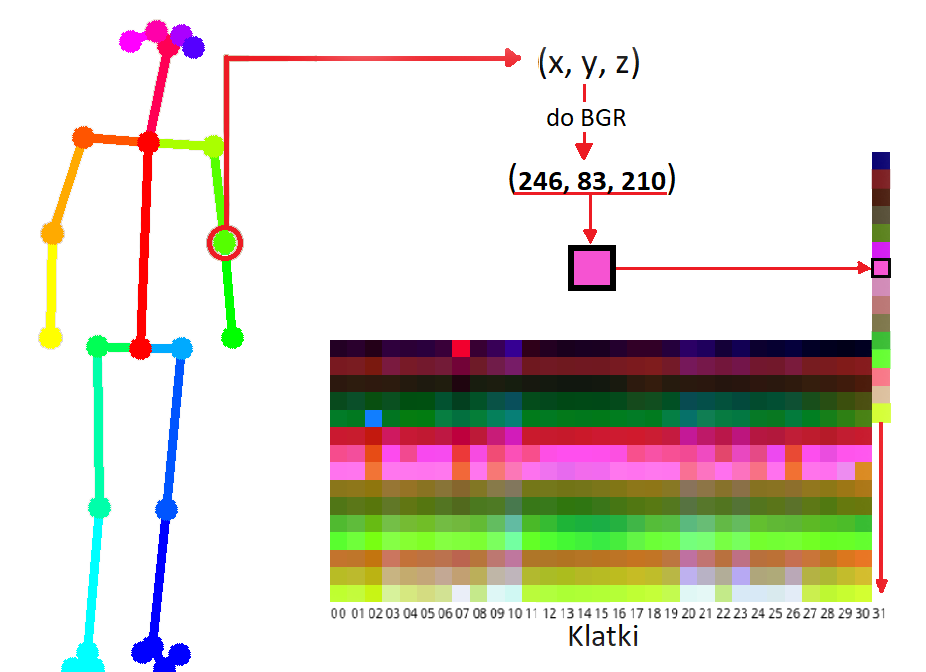
\includegraphics[width=0.6\textwidth]{./images/Classificators/MMakos_image_prep}
	\caption{Преобразование данных в модели от M. Makos. \cite{mmakos}}
	\label{fig:mmakos_image_prep}
\end{figure}
\hspace{1cm}

Для классификации используется версия сети VGG. По решению автора все позы делятся на два супер-класса: динамические и статические, а потом уже классифицируются внутри супер-классов более точно.



\subsubsection{MMaction2 by OpenMMlab}
\label{subsubsec:mmaction2_desc}

MMAction2 является подпроектом лаборатории Open-MMLab \cite{2020mmaction2}. Идея классификации движения начиналась с проекта MMSkeleton построенном на исследовании про ST-GCN \cite{STGCN} и позже переросло в первую версию MMAction для классификации движений одного человека. Текущая версия может обрабатывать взаимоотношения между людьми, такие как обнимания или рукопожатия. 

Для классификации необходимо сначала обработать видеофрагмент. Для этого производится поиск и локализация действия во времени, а также восстановление и анализ скелета.

В первом случае используется TimeSformer \cite{TimeSformer} - создан на основе идеи Transformer для обработки видеопотоков. Он использует несколько видов блоков Attention (см. \autoref{fig:timesformer}) для объединения информации на нескольких кадрах до и после текущего. Это дает возможность точно распознавать действия в кадре и отслеживать их.

\begin{figure}[h]
	\centering
	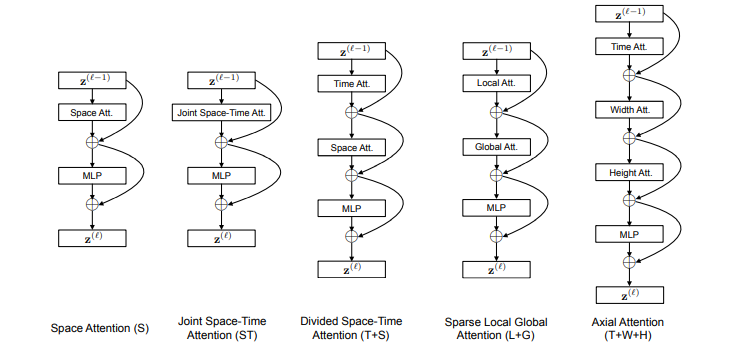
\includegraphics[width=0.9\textwidth]{./images/Classificators/TimeSformer}
	\caption{Примеры блоков внимания в TimeSformer. \cite{TimeSformer}}
	\label{fig:timesformer}
\end{figure}

Для обработки скелетов используется модель PoseC3D \cite{duan2021revisiting}. Она использует несколько тепловых 3D-карт в качестве представления скелета человека и за счет этого обходит GCN и более устойчив к шумам на изображении. Также без особенно лишних затрат можно использовать PoseC3D для классификации взаимодействия между людьми.

\begin{figure}[h]
	\centering
	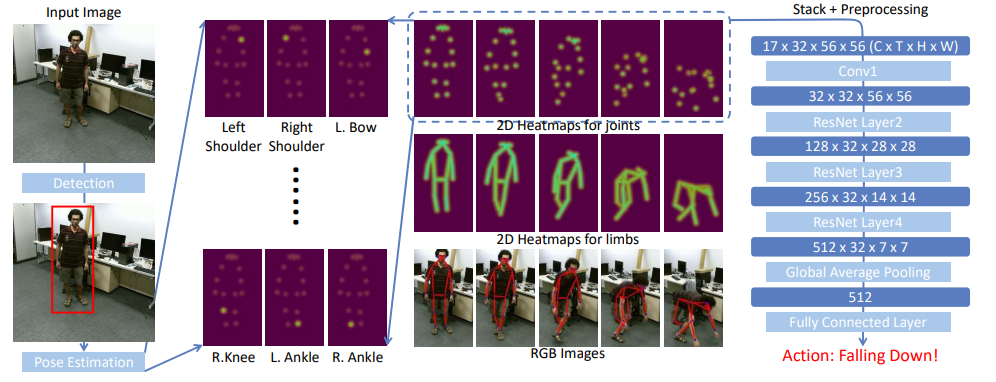
\includegraphics[width=\textwidth]{./images/Classificators/PoseC3D}
	\caption{Структура сети PoseC3D. \cite{duan2021revisiting}}
	\label{fig:posec3d}
\end{figure}

Все исследования проекта основаны на классификации и анализе видео, что полезно для будущих исследований и развитии темы работы.


\newpage